\documentclass{article}
\usepackage[utf8]{inputenc}
\usepackage[icelandic]{babel}
\usepackage[T1]{fontenc}
\usepackage{graphicx}
\usepackage{mathtools}
\usepackage{amsmath}
\usepackage{amssymb}
\usepackage{minted}
\usepackage{listings}


\graphicspath{ {./} }
\title{Vikublað 10 - tölvunarfræði 2}
\author{ttb3@hi.is}
\date{\today}


\begin{document}
\maketitle

\section*{4.1.14}
BFS notar \emph{queue} til að geyma upplýsingar um hnúta sem búið er að skoða.
Þetta gerir BFS kleift að finna stysta veg á milli tveggja hnúta.
Ef við myndum nota \emph{stack} myndi það hafa áhrif á leitina á þann hátt að öll önnur hliðin væri farin áður en byrjað væri að skoða hina.
Frekar illa orðað en sjá teikningar,
\begin{center}
    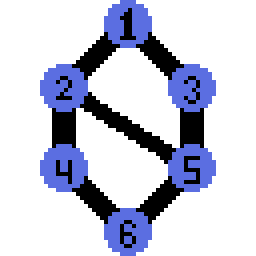
\includegraphics{graph.png}
\end{center}
Ef við byrjum með þetta tré og förum snöggt í gegnum það hvernig leitað væri í því með BFS þar sem er notað \emph{queue}.
Q táknar queue, P táknar print. Hver lína felur í sér að prenta næsta hnút í röðinni og setja tengda hnúta í röðina. Við byrjum á 1.\\
\begin{center}
    \begin{tabular}{|l|l|}
        \hline
        P&Q\\
        \hline
                    &1\\
                    \hline
        1           &2,3\\
        \hline
        1,2         &3,4,5\\
        \hline
        1,2,3       &4,5\\
        \hline
        1,2,3,4     &5,6\\
        \hline
        1,2,3,4,5   &6\\
        \hline
        1,2,3,4,5,6 &\\
        \hline
    \end{tabular}
\end{center}

Sjáið núna muninn ef við notum \emph{stack} en ekki \emph{queue}:
\begin{center}
    \begin{tabular}{|l|l|}
        \hline
        P&Q\\
        \hline
        &1\\
        \hline
        1&2,3\\
        \hline
        1,3&2,5\\
        \hline
        1,3,5&2,6\\
        \hline
        1,3,5,6&2,4\\
        \hline
        1,3,5,6,4&2\\
        \hline
        1,3,5,6,4,2&\\
        \hline
    \end{tabular}
\end{center}
Sama niðurstaða og við fengjum með DFS, þannig tldr. ef við notum \emph{stack} í stað \emph{queue} í BFS er ekki hægt að fá stystu leið því við erum í raun bara að nota DFS.

\section*{Bacon Tala}
hérna er forritið sem ég notaði til þess að finna tölurnar:

\begin{lstlisting}
    import edu.princeton.cs.algs4.*;

    public class Bacon {
        public static void main(String[] args) {
            SymbolGraph sg = new SymbolGraph(args[0], args[1]);
            Graph G = sg.graph();
            String source = args[2];
            if (!sg.contains(source)) {
                StdOut.println(source + " not in database.");
                return;
            }
            int s = sg.indexOf(source);
            BreadthFirstPaths bfs = new BreadthFirstPaths(G, s);
            while (!StdIn.isEmpty()) {
                String sink = StdIn.readLine();
                if (sg.contains(sink)) {
                    int t = sg.indexOf(sink);
                    int c = 0;
                    if (bfs.hasPathTo(t)) {
                        for (int v : bfs.pathTo(t)) {
                            StdOut.println(" " + sg.nameOf(v));
                            c++;
                        }
    
                        System.out.println("c --> " + (c-1)/2);
                    } else
                        StdOut.println("Not connected");
                } else
                    StdOut.println("Not in database.");
            }
        }
    }
    
\end{lstlisting}

\end{document}